\chapter{相关技术与理论基础}

\section{词向量表示}

词嵌入(Word embedding)是文档词汇最流行的表示形式之一,它是特定单词的向量表示,它能够捕获文档中单词的上下文,语义和句法相似性,与其他单词的关系等。
Word2Vec是使用浅层神经网络学习单词嵌入的最流行技术之一,它是由Tomas Mikolov于2013年在Google上提出的。
Word2Vec是一个浅层的两层神经网络,经过训练可以重建单词的上下文语义。 它的输入来源是一个大的单词语料库,通常产生一个具有几百个维度的向量空间,
该语料库中的每个唯一单词都在该空间中分配了一个相应的向量。 词向量位于向量空间中,以便在语料库中共享公共上下文的词在空间中彼此紧邻。 
Word2Vec是一种从原始文本中学习单词嵌入的计算效率特别高的预测模型,
它主要有两种方式,连续词袋(CBOW)模型和Skip-Gram模型,如图\ref{fig:word2vec_diagrams}。

\begin{figure}[htbp]
    \centering
    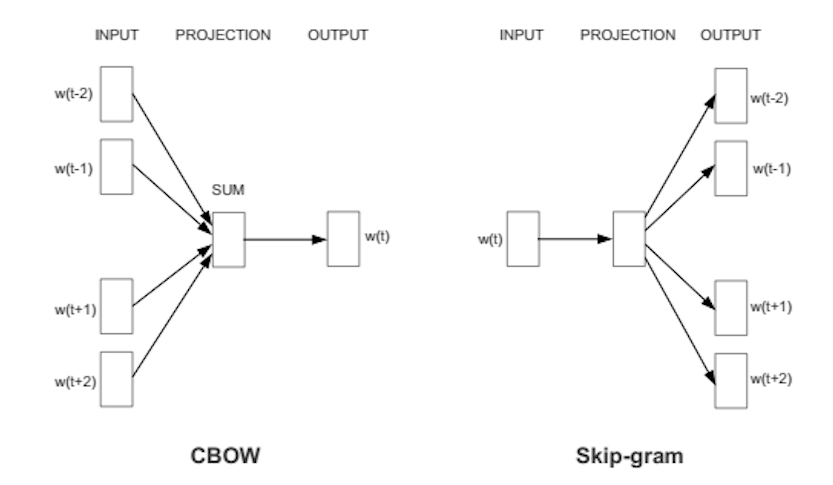
\includegraphics[scale=0.5]{./images/word2vec_diagrams.png}
    \caption{word2vec两种训练方式}
    \label{fig:word2vec_diagrams}
  \end{figure}

  Word2Vec是具有单个隐藏层的简单神经网络,并且像所有神经网络一样,它具有权重,并且在训练过程中,其目标是调整这些权重以减少损失函数。 
  但是,Word2Vec不是用于他训练时处理的任务,相反,我们将仅使用其隐藏的权重,将其用作词嵌入,然后将模型的其余部分扔掉。